\documentclass[convert={size=400x1300,outext=.jpg},class=minimal,border=0mm]{standalone}
\usepackage{tikz}
\usetikzlibrary{backgrounds}
\usetikzlibrary{patterns}
\begin{document}
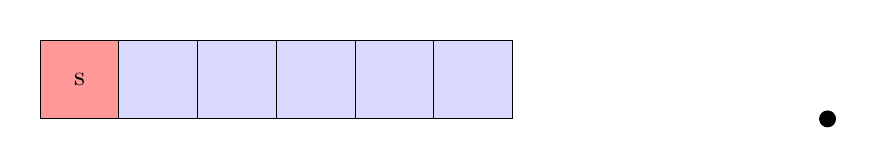
\begin{tikzpicture}[ show background rectangle, background rectangle/.style={fill=white} ]

	\tikzstyle{fractional}=[fill=red!40]
	\tikzstyle{integer}=[fill=blue!15]
	\tikzstyle{sign}=[fill=purple!15]

	%FPF=(9,4)
	\draw (-10.000000,0.000000) rectangle ++(1,1) [fill=red!40,] node[midway] {s};
	\draw (-9.000000,0.000000) rectangle ++(1,1) [fill=blue!15,] node[midway] {};
	\draw (-8.000000,0.000000) rectangle ++(1,1) [fill=blue!15,] node[midway] {};
	\draw (-7.000000,0.000000) rectangle ++(1,1) [fill=blue!15,] node[midway] {};
	\draw (-6.000000,0.000000) rectangle ++(1,1) [fill=blue!15,] node[midway] {};
	\draw (-5.000000,0.000000) rectangle ++(1,1) [fill=blue!15,] node[midway] {};
	\draw[black,fill] (0,0.000000) circle [radius=0.1cm];


\end{tikzpicture}
\end{document}